\noindent \scalebox{0.8}{\textit{Reference: \cite{lubanovic2019introducing} Chapter 7}}

In this chapter we introduce lists and this occasions the discussion of a new idea, (im)mutability. We cover just the basics to help prepare us for for loops. % and iterable


\section{Defining Lists}

We have worked with strings, integers, floats, and booleans so far. Now, we introduce a compound data type the list.
Lists are also a sequence object, meaning they are ordered. 

A list is constructed by separating one or more objects with commas and placing them in square brackets. For example, 
we can define a list as 

\begin{lstlisting}[language = Python]
# Our first list
floor = ['yoga', 'meditation', 'stretching', 'strength', 'cardiovascular'] \end{lstlisting}


\smallskip

\begin{lstlisting}[language = Python]
# More lists
aquatic = []
cycling = ['cycling'] \end{lstlisting}

Above, \code{[]} created an empty list. You could also use, and you might prefer \code{list()}. The reason you might prefer \code{list()} is because explicit is better than implicit\footnote{From the Zen of Python.}, and this makes it explicit that you're creating a list.
\smallskip

\begin{lstlisting}[language = Python]
# More lists
treadmill_based = ['running','walking','bootcamp']  \end{lstlisting}

\smallskip

A useful quality of lists is that they can be of mixed type. 


\begin{lstlisting}[language = Python]
# More lists
fine_list = [0, 'milk', cycling]  \end{lstlisting}

\subsection{Indexing, Slicing, Mutating}

You can obtain the element at a certain place, or \emph{index}, in a list by suffixing the list with that index number inside square brackets. 
Python uses zero-based indexing. So the $n^{\text{th}}$ item is at index $n-1$.


\begin{lstlisting}[language = Python]
# Get specific items
fine_list = [0, 'milk', cycling]

# Which of these print statements will raise an error?
print(fine_list[0])
print(fine_list[1])
print(fine_list[2])
print(fine_list[3])
print(fine_list[-1])) \end{lstlisting}



\smallskip
\noindent We can also count from the end of the list to find an item, as hinted by the 
\lstinline[language=Python]{fine_list[-1]} above. The index $-1$ will identify the last element. So, in some sense, you might think that negative indexing
is not zero-based. If that's confusing, just recall $-0 = 0$ and so \lstinline[language=Python]{fine_list[-0]} 
is actually the same as \lstinline[language=Python]{fine_list[0]}.


\smallskip

\noindent The following graphic helps explain how lists (and strings) are indexed.

\begin{figure}[h!] 
\begin{center} 
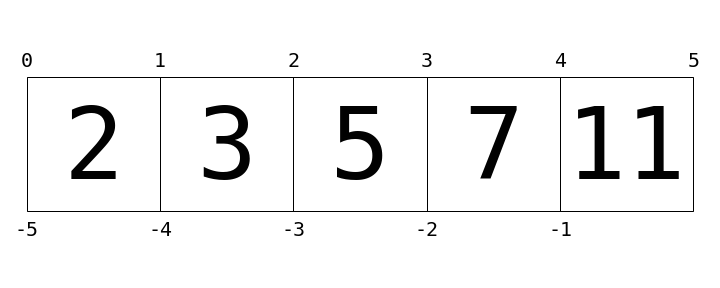
\includegraphics[width = .55\textwidth]{list_indexing.png}
\caption{Indexing (\link{https://jakevdp.github.io/WhirlwindTourOfPython/06-built-in-data-structures.html}{From \cite{vanderplas2016whirlwind}}).}
\label{fig:while}
\end{center}
\end{figure}


%% Slicing

\bigskip

\noindent While indexing pulled out a single element, we can also \emph{slice} to pull out a sublist. 


\begin{lstlisting}[language = Python]
# Get specific items
['Jack', 'Jill', 'and', 'hill', 'over', 'ran', 'the']
print(fine_list[0:2])
print(fine_list[-2:]) \end{lstlisting}

\noindent The first print statement will print elements 0 and 1 in a list. The last print statement will print a list of just the last two elements. Why is slicing done this way? Why does the numbering start at zero and why is the upper bound excluded? It's more of a computer science convention than a Python-specific one. \cite{ramalho2015fluent} (freely downloadable from Columbia Library) addresses this on page 33 and Dijkstra provides some reasoning \link{https://www.cs.utexas.edu/users/EWD/transcriptions/EWD08xx/EWD831.html}{here}. Those reasons are basically:
\begin{enumerate}
    \item The length of the list is more obvious. \code{fine_list[0:2]} contains 2-0=2 elements. And \code{fine_list[:4]} contains four elements. 
    \item It's easy to partition a list. \code{fine_list[:3]} and \code{fine_list[3:]} don't overlap. 
\end{enumerate}



%% Mutability 
\bigskip

\index{mutability}
\noindent Lists are \emph{mutable}, meaning that we can change their contents.

\begin{lstlisting}
# Friend drama
my_best_friends = ['Richard', 'Spiro']
print(my_best_friends)
my_best_friends[1] = 'Gerald'
print(my_best_friends)
\end{lstlisting}


Mutability has consequences when you are assigning one variable to be equal another. By changing \code{b}, which is made from \code{a}, we also change \code{a}. 

\begin{lstlisting}
a = [1,3,5]

b = a
b[2] = 99

print(a)
print(b)
\end{lstlisting}

This was \emph{not} the case for immutable objects like integers, floats, and strings. 

\begin{lstlisting}
a = 1
b = a
a += 1

# b and a are not the same
print(a)
print(b)
\end{lstlisting}



However, we don't see the same effect on mutable objects when reassigning them. 

\begin{lstlisting}
a = [1,3,5]

b = a
b = b[0:1]

# b and a are no longer pointing to the same list
print(a)
print(b)
\end{lstlisting}

Just when ``mutating'' them. 

\begin{lstlisting}
a = [1,3,5]

b = a
b = b.append(7)

# b and a are pointing to the same list
print(a)
print(b)


# This also does the same
a = [1]
b = a

a += [1]

# b and a are pointing to the same list
print(a)
print(b)
\end{lstlisting}